\chapter{The CMS Detector}
The Large Hadron Collider (LHC) is a particle accelerator and collider located in a 26.7 km tunnel underneath Geneva, Switzerland~\cite{Evans_2008}. The LHC is designed to operate at center-of-mass energies up to $\TeV{14}$, although these energies have only been reached recently. Protons can reach these energies more easily than electrons, which the predecessor to the LHC collided, because they lose relatively less energy when they are accelerated. The LHC consists of two rings with beams moving in opposite directions. These rings cross over at four different interaction points, where the main detectors at the LHC are positioned. Owing to the $\SI{3.7}{\m}$ diameter of the tunnel, there is not enough space for two separate magnet rings and instead a two-bore magnet is used. This magnet, comprised of niobium-titanium superconductors, is cooled to $\SI{2}{\kelvin}$ by superfluid helium to maintain a magnetic field of $\SI{8}{\tesla}$. This allows for the high-energy proton-proton collisions necessary for the work of the main detectors. 

At the LHC, the number of events per second is given by 
\begin{equation}
    N_\text{event} = L\sigma_\text{event}
\end{equation}
where $\sigma_\text{event}$ is the cross-section of the event and $L$ is the luminosity. The luminosity itself can be expressed in terms of parameters of the beam as
\begin{equation}
    L = \frac{N_b^2n_bf_\text{rev}\gamma_r}{4\pi\epsilon_n\beta^*}F
\end{equation}
where $N_b$ is the number of particles per bunch (a grouping of protons in the beam), $n_b$ is the number of bunches per beam, $f_\text{rev}$ is the frequency of revolution, $\gamma_r$ is the Lorentz factor, $\epsilon_n$ is the normalized transverse beam emittance, $\beta^*$ is the Beta function at the collision point, and $F$ is percentage by which the luminosity is reduced due to the beam crossing angle $\theta_c$. The current operating luminosity of the LHC is around $\SI{2d34}{\cm^{-2}\s^{-1}}$.

In order to increase the amount of data collected by the detectors in the LHC, the collider is being upgraded to increase the luminosity~\cite{Contardo:2020886}. The magnets that focus the beams in the LHC will be replaced and the bunch overlap in the optimization region will be optimized. This will allow the luminosity to increase to a maximum of $\SI{2d35}{\cm^{-2}\s^{-1}}$, although the typical operating luminosity will be $\SI{5d34}{\cm^{-2}\s^{-1}}$. This will increase the PU from 25 to 140 under mean conditions, with a peak of 200.

\section{The CMS Detector}
One of the main detectors at the LHC is the Compact Muon Solenoid (CMS). The technical specifications of CMS are summarized below. For a more in-depth description of the detector, see~\cite{Collaboration_2008}. \cref{fig:cms} presents a schematic view of the detector.

\begin{figure}[ht]
    \centering
    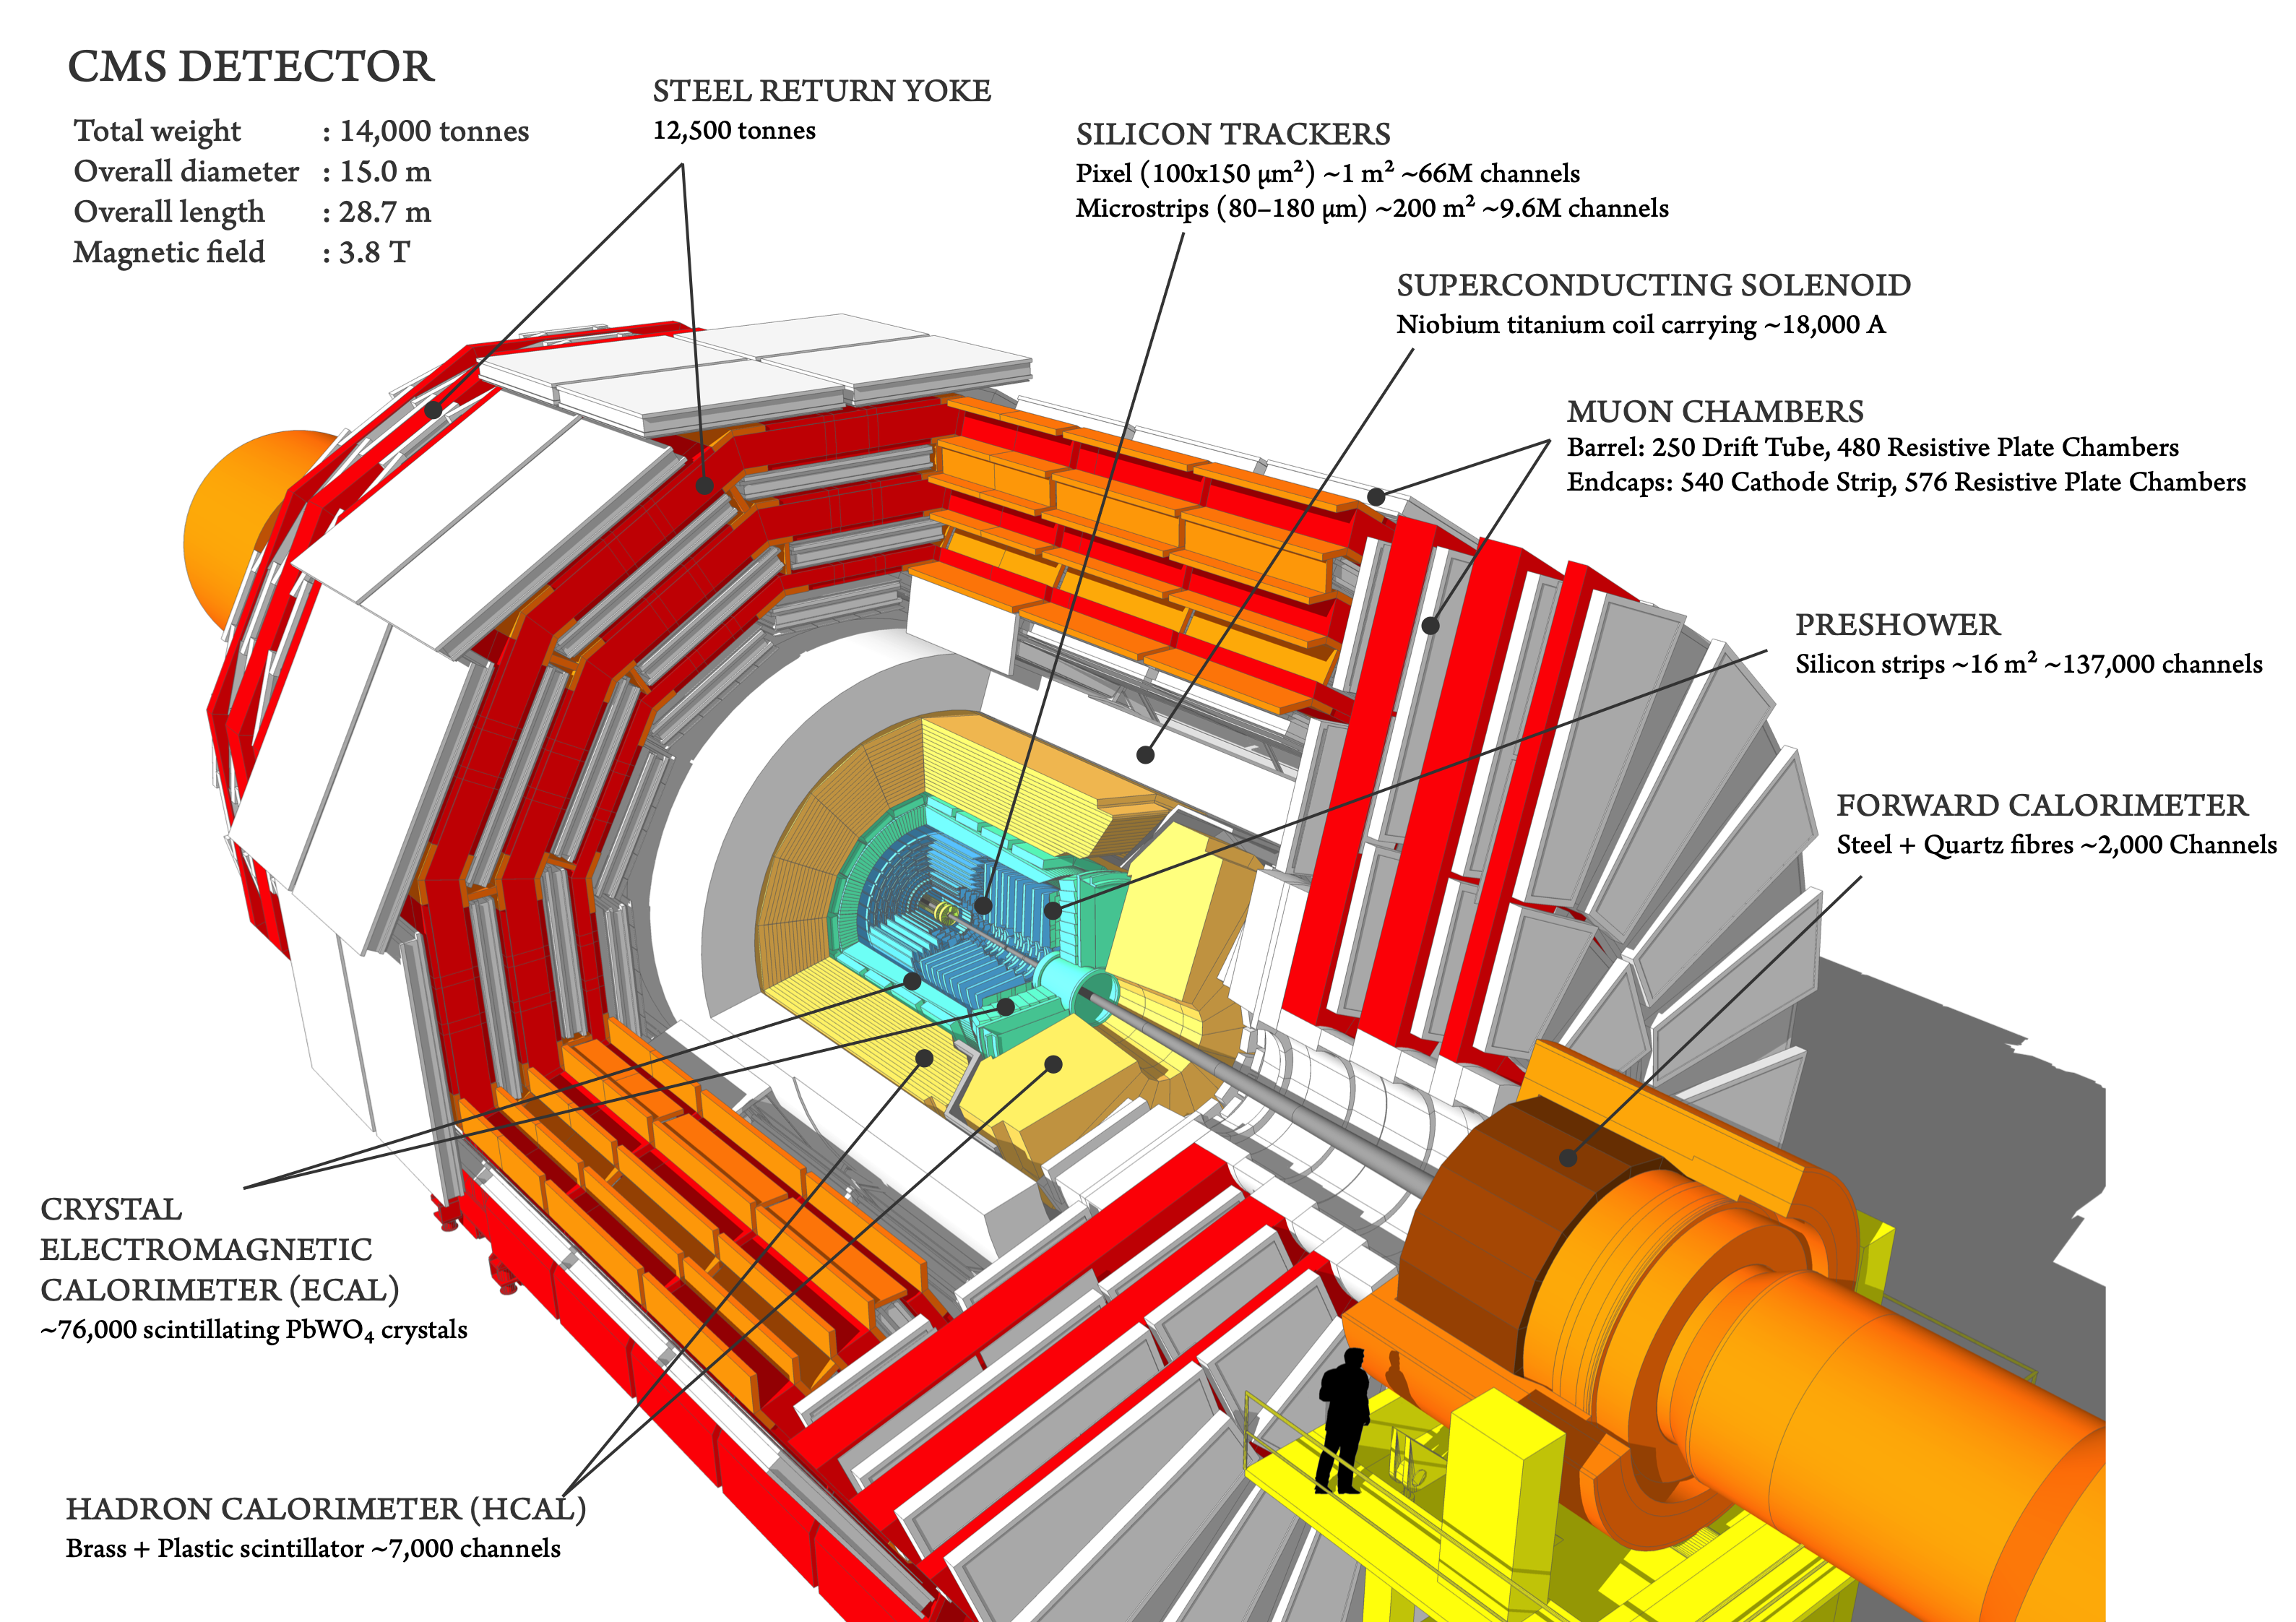
\includegraphics[width=0.75\textwidth]{Chapters/CMS/cms_160312_02.png}
    \caption{The CMS detector at the LHC in CERN~\cite{Sakuma_2014,Sakuma:2665537}.}
    \label{fig:cms}
\end{figure}

The main part of the CMS detector is $\SI{21.6}{\m}$ long and $\SI{14.6}{\m}$ in diameter, with a total weight of around $12500$ metric tons. The central feature of the detector is the titular solenoid, which can provide magnetic fields of strength up to $\SI{4}{\tesla}$. The superconducting magnet is $\SI{12.5}{\m}$ long with a diameter of $\SI{6}{\m}$. The main function of the solenoid is to cause charged particles in the detector to curve, allowing for measurement of their charge and momentum. Inside of the solenoid are the silicon tracker, the electromagnetic calorimeter (ECAL) and the hadron calorimeter (HCAL). Outside of the solenoid are a system of detectors designed for identifying and determining the properties of muons. Information from all these systems is taken by the CMS trigger for further processing before being stored. 
In the detector, the $y$-axis points vertically upward, the $x$-axis points radially inward towards the center of the LHC, and the $z$-axis points in the beam direction. The typical coordinates used for tracking objects in the detector are the angle $\phi$ from the $x$-axis in the $x$-$y$ plane, the distance $r$ in the $x$-$y$ plane, and the pseudorapidity $\eta$ measured as $\ln\tan(\theta/2)$, where $\theta$ is the polar angle measured from the $z$-axis.
It is common to refer to distances in the detector using the variable $R$, which is equal to $\sqrt{\eta^2+\phi^2}$.
The transverse components of the energy and momentum are calculated from the $x$ and $y$ components.

The innermost component of the detector is the tracker, which is $\SI{5.8}{\m}$ long and $\SI{2.5}{\m}$ in diameter. In the barrel of the solenoid, the tracker has three layers of silicon pixel detectors, followed by ten layers of silicon micro-strip detectors. Four of those layers comprise the tracker inner barrel (TIB) with thinner strips, while the remaining six are the tracker outer barrel (TOB) with thicker strips. The endcaps of the pixel detector have two disks of pixel detectors, while each endcap of the TIB have three disks of silicon strips. Lastly, there are nine endcap disks of silicon strips that bookend the entire tracker. Signals from the silicon detectors are read out by a sequence of chips.
The silicon tracker is able to measure vertex information and the \pt of physics objects with high precision and granularity. For high-momentum tracks, the latter can be measured with a resolution of 1-2\% up to $|\eta| = 1.6$. Although information from the tracker is not fed into the level-one (L1) trigger, it is part of the high-level trigger (HLT).

Moving radially outward, the next section of the detector is the electromagnetic calorimeter (ECAL). The ECAL is comprised of lead tungstate crystals. There are approximately 61000 of these crystals in the barrel of the ECAL, which covers a pseudorapidity of $|\eta| < 1.479$. There are around $7000$ crystals in each endcap, which cover the pseudorapidities between $|\eta| = 1.479$ and $|\eta| = 3.0$. When an electromagnetic particle passes though the ECAL, the crystals scintillate. The photons from these scintillations are detected by silicon avalanche photodiodes (APDs) in the barrel and by vacuum phototriodes (VPTs) in the endcaps. The ECAL electronics then report the energy deposited in a five-by-five section of the ECAL called a tower. Because the intensity of the scintillation is dependent on the temperature of the crystals, the ECAL is kept at $\SI{18}{\degreeCelsius}$.

Between the ECAL and the solenoid is the hadron calorimeter (HCAL). The HCAL is comprised of layers of brass absorbers and scintillating materials. Particles that hit the brass absorbers create a shower of secondary particles that cause the scintillators to emit photons. These photons are then detected by hybrid photodiodes (HPDs). The barrel of the HCAL (HB) covers up to $|\eta| = 1.3$. It is split into two halves with a total of 36 wedges, each of which are divided further into 4 $\phi$ sections. The endcap of the HCAL (HE) covers $1.3 < |\eta| < 3.0$. Because of the limited space between the ECAL and solenoid, in addition to the HB and HE, there is also a calorimeter outside the solenoid called the outer calorimeter (HO). The final piece of the HCAL is the forward calorimeter (HF) which extends the pseudorapidity range up to $|\eta| = 5.2$. The HF uses quartz fibers as its scintillators, whose photons are then read by photomultiplier tubes (PMTs).

The final major detector system is the set of detectors focused on identifying muons, determining kinematic information such as their \pt, and feeding information to the trigger. The muon system is a key part of CMS, as many important processes have muon final states. The barrel region of the muon system is comprised of drift tube (DT) chambers. There is not as much muon or background activity in the barrel, but closer to the beam the rate of activity increases, necessitating the use of the more precise cathode strip chambers (CSCs). In addition to being more segmented, the CSCs also fire faster than the DTs and are more resistant to radiation. The CSCs are used for pseudorapidities $0.9 < |\eta| < 2.4$. The CSCs are comprised of 6 anode wire plates which are sandwiched between 7 cathode wire plates. Particles that hit the anodes cause a shower of electrons which are drawn to the cathodes. The final muon subsystem is the resistive plate chambers (RPCs) which are present in both the barrel and endcaps, encompassing $|\eta| < 1.9$. The RPCs add additional information by being fast to respond, giving clear timing information. However, they are spatially coarser than the other detectors.

The information gleaned by the detector systems is fed into the triggers. Owing to the vast quantity of events taking place in the detector, most of these events cannot be stored. The trigger determines which of these events should be read out. The first trigger level is the level-one (L1) trigger, which is comprised of hardware in the detector systems. After events are processed by the L1 trigger, the high-level trigger (HLT) uses software to further determine which events should be stored offline. 
The L1 trigger begins with local triggers from energy deposits in the calorimeters and track hits in the muon chambers. This information is then fed into the regional triggers, which form particle object candidates and rank them. The regional muon trigger (RMT) determines tracks from the segments in the muon system, while the regional calorimeter trigger (RCT) determines electron and photon candidates, calculates some information for the muon candidates, and determines the tau veto. The global muon trigger takes information from the regional muon triggers to create muon candidates. The global calorimeter trigger creates jet candidates using a clustering technique. It also calculates global properties such as $E_\mathrm{T}$, \ptmiss, and $H_\mathrm{T}$. Information from this trigger level is fed into the global trigger, which determines which events to reject and which to forward to the HLT. 
The HLT takes on a wider array of information than the L1 trigger, allowing it to perform calculations similar to those done in offline analysis. This further reduces the number of stored events by not reading events with few valid or interesting candidates.

\section{CMS Phase-2}
\label{section:phase2}
In order to facilitate the taking of data during the HL-LHC era, CMS will undergo a series of upgrades referred to as CMS Phase-2. The overall goal of the upgrades is to ensure that the detector can handle the increase in pileup and radiation from the increased luminosity.

The L1 trigger will have its rate increased to $\SI{750}{kHz}$ and its latency increased to $\SI{12}{\us}$~\cite{CERN-LHCC-2020-004}. The HLT will have an upgraded rate of $\SI{7.5}{kHz}$.

The tracker system of CMS will be replaced entirely due to the high amount of radiation that will occur during Phase-2~\cite{CERN-LHCC-2017-009}. In place of the old tracker there will be an Outer Tracker (OT) that will help provide tracking information to the L1 trigger by rejecting tracks below a certain \pt. This will be done using \pt modules comprised of either two strip sensors or a strip and a macro-pixel sensor. These modules must be radiation resistant, due to the increased luminosity at the HL-LHC. The Inner Tracker (IT) will be comprised of thin silicon pixels that are designed for the increased radiation tolerance and granularity required of the Phase-2 IT. The IT is designed to be replaceable during shutdowns, due to the high amount of radiation damage that it will incur. Owing to the trigger upgrades described earlier, the tracker electronics will also be upgraded to work with those upgrades and allow for input from the tracker to the L1 trigger. Finally, the geometry of the tracker will be enhanced, allowing tracking up to pseudorapidities around $|\eta| = 4$.

Further improvements to CMS will occur in the barrel. As in the tracker, the electronics of the electromagnetic calorimeter (ECAL) will be upgraded to function with the improved trigger~\cite{CERN-LHCC-2017-011}. In particular, the L1 trigger will receive information from the individual lead tungstate crystals, as opposed to from the towers, to enable better track matching. The electronic upgrades, along with cooling the ECAL from $\SI{18}{\degreeCelsius}$ to $\SI{9}{\degreeCelsius}$, will also reduce the noise in the ECAL. The hadronic calorimeter (HCAL) will also have its electronics upgraded for compatibility with the trigger. The endcap calorimeters will be replaced by the HGCAL, which will be designed to withstand the heavier radiation of the HL-LHC~\cite{CERN-LHCC-2017-023}. 

As with the other CMS systems, the muon system electronics must be upgraded to function with the improved trigger~\cite{CERN-LHCC-2017-012}. Additionally, the geometric acceptance of the muon system will be increased to around $|\eta|=2.8$ by use of resistive plate chambers (RPCs) and gas electron multipliers (GEMs).

The final main upgrade to CMS is the inclusion of a minimum ionizing particle timing detector (MTD)~\cite{CMS:2667167}. In order to mitigate the effects of the increased PU of the HL-LHC, it is useful to be able to differentiate vertices not just in space but also in time. The MTD is split into two regions: the Barrel Timing Layer (BTL) covering $|\eta| < 1.5$ between the OT and the ECAL and the Endcap Timing Layer (ETL) covering $1.6 < |\eta| < 3.0$ in front of the endcap calorimeter. The BTL will consist of scintillating cerium-doped lutetium-yttrium oxyorthoscillicate crystals read out by silicon photomultipliers. The ETL will use silicon devices that can better withstand the radiation in the endcaps. The MTD will have a timing resolution of $\SI{30}{\ps}$ that comes from the detection of two hits per track in the various detection devices.
